\documentclass[12pt]{article}
\usepackage{url,graphicx,tabularx,array,geometry}
\usepackage[utf8]{inputenc}
\usepackage{hyperref}
\usepackage{listings}
\usepackage{setspace}

\setlength{\parskip}{1ex} %--skip lines between paragraphs
\setlength{\parindent}{0pt} %--don't indent paragraphs

%-- Commands for header
\renewcommand{\title}[1]{\textbf{#1}\\}
\renewcommand{\line}{\begin{tabularx}{\textwidth}{X>{\raggedleft}X}\hline\\\end{tabularx}\\[-0.5cm]}
\newcommand{\leftright}[2]{\begin{tabularx}{\textwidth}{X>{\raggedleft}X}#1%
& #2\\\end{tabularx}\\[-0.5cm]}
\onehalfspacing
%\linespread{2} %-- Uncomment for Double Space
\begin{document}

\title{Robotics Project  Autumn 2013}
\line
\leftright{\today}{Alexander Rüedlinger, 08-129-710, Group 01} %-- left and right positions in the header
\section*{Series 2}
\paragraph{Exercise}
If you run into any troubles, describe your problem and upload it to \\
\url{http://www.diuf.unifr.ch/pai/pr1} as a .pdf file.

\subsection*{Our troubles}
Unfortunately our group 01 couldn't connect the e-pucks with aseba studio.

Me and my group partner, we tried to follow the instructions on the "Connection Guide" sheet to connect the e-pucks with aseba studio. We double checked each step and we're are convinced that we followed the steps from 1 to 8 correctly. Unfortunately, we were stuck in step 9 on the guide.

\subsubsection*{Trouble 1}

The first problem we ran into is the missing aseba studio desktop link on both ubuntu machines.

Step 9 in the connection guide says:
\begin{quote}
[...]Step 9: Now we are ready to start ASEBA Studio by clicking on the icon Aseba Studio on the desktop.[...] 
\end{quote}

Should there be a special desktop link with pre-configured values to start aseba studio?

\subsubsection*{Trouble 2}
Despite the missing desktop link, we started aseba studio using the ubuntu unity interface by entering 'aseba' and clicking on the found aseba studio icon. 

Here, we encounterd the following dialog and we didn't know which settings were required to connect the e-pucks via bluetooth.
\begin{figure}[!htb]
\centering
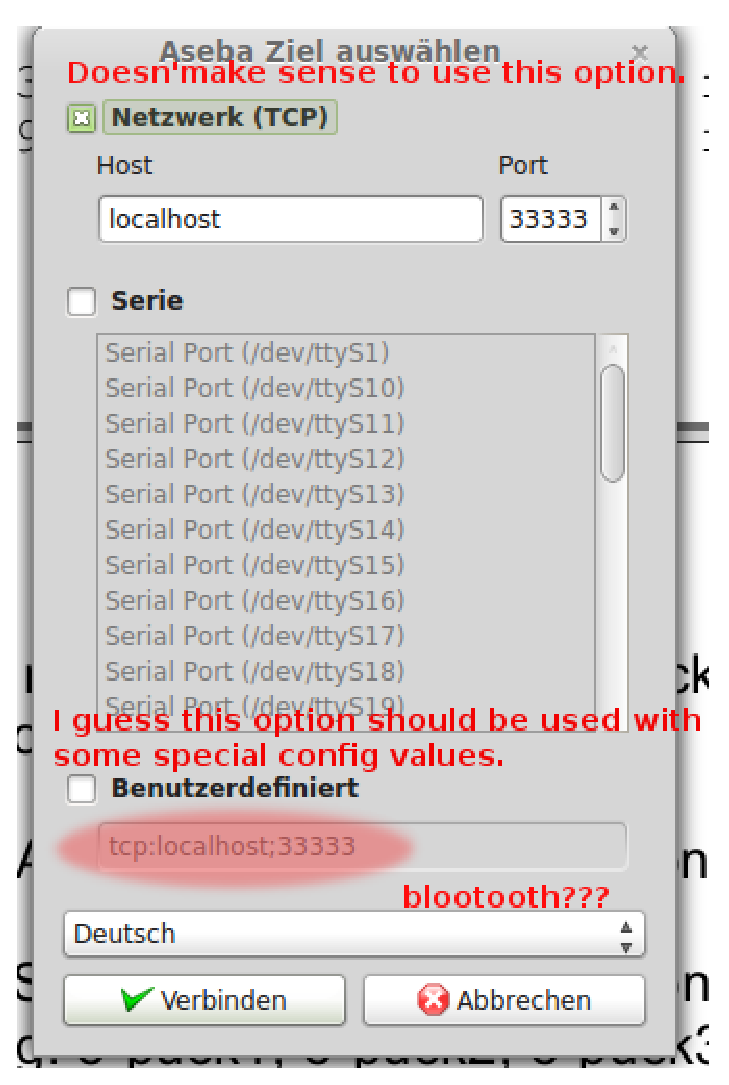
\includegraphics[scale=0.5]{aseba.eps} 
\caption{Starting aseba studio}
\end{figure}

We tried different settings, but everytime we started aseba there were no tabs visible for each successfully connected e-puck.

\subsection*{What we've accomplished}
\subsubsection*{Step 1 - 2}
The figure below shows four e-pucks. The green light on each e-puck indicates that the battery are put in correctly and that thet e-pucks are ready to use.
\begin{figure}[!htb]
\centering
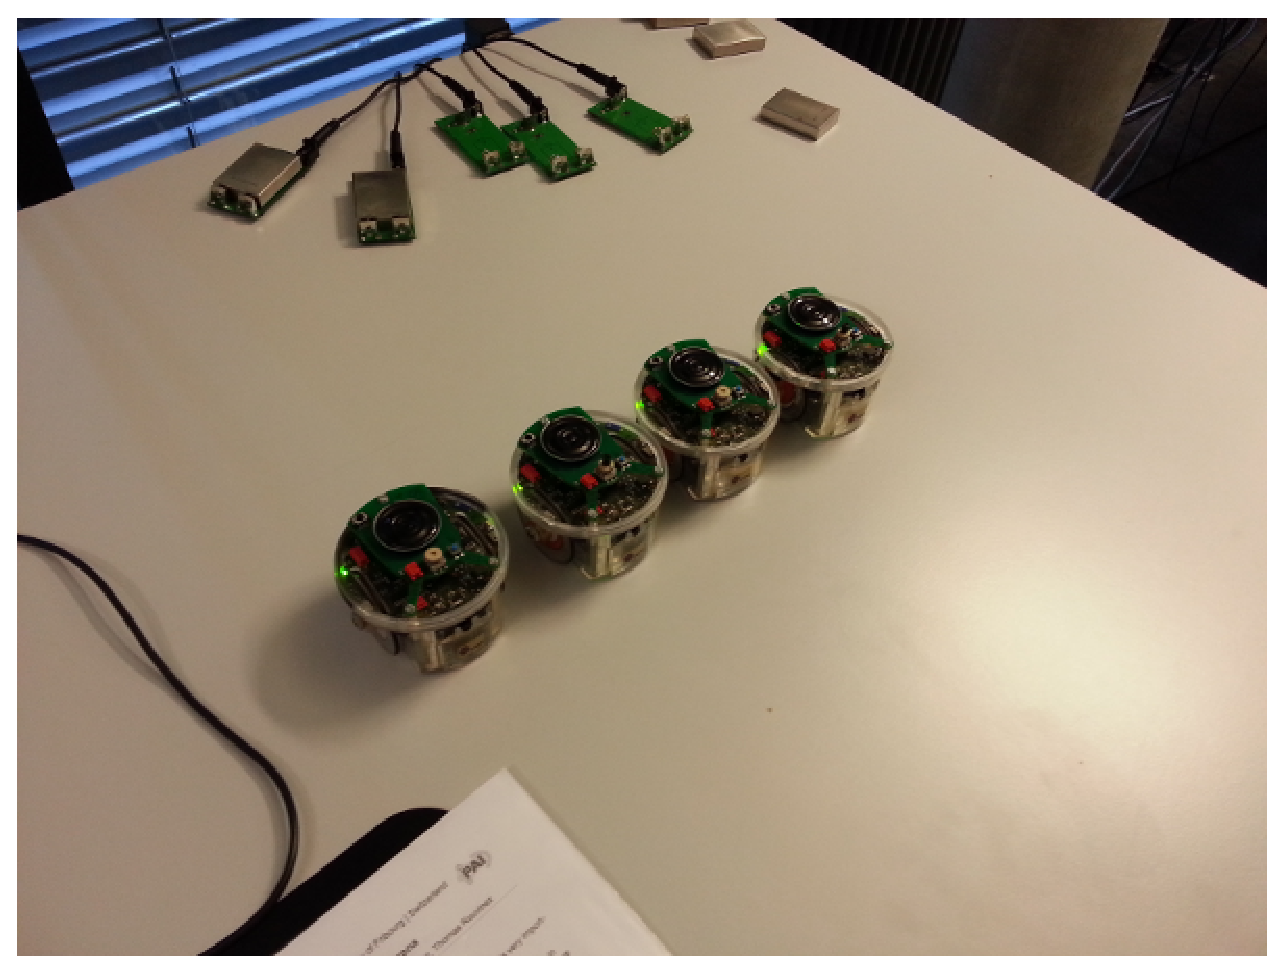
\includegraphics[scale=0.5]{pics/epucks_1.eps} 
\end{figure}

\subsubsection*{Step 3 - 5}
In the following steps we used only two e-pucks.

Using the hcitool scann command we searched for all connectable bluetooth devices:
\begin{lstlisting}
hcitool scan

Scanning ...
	10:00:E8:52:BB:D5	e-puck_1466
	10:00:E8:52:BF:55	e-puck_1471
	00:22:41:D5:9C:70	robotics1-0
\end{lstlisting}

As we can see two e-pucks were found.

\subsubsection*{Step 6 - 8}
In step 6 we connected each e-puck using the rfcomm bind command:
\begin{lstlisting}
sudo rfcomm bind 0 10:00:E8:52:BB:D5
sudo rfcomm bind 1 10:00:E8:52:BF:55
\end{lstlisting}

In step 7 we established a connection between aseba studio and the previous created rfcomm bindings.

We got the following output on the terminal:
\begin{lstlisting}
asebaswitch -v ser:device=/dev/rfcomm0 ser:device=/dev/rfcomm1

[Tue Sep 24 13:21:50 2013 270] Incoming connection from 
ser:device=/dev/rfcomm0;baud=115200;stop=1;parity=none;fc=none;bits=8
[Tue Sep 24 13:21:54 2013 277] Incoming connection from 
ser:device=/dev/rfcomm1;baud=115200;stop=1;parity=none;fc=none;bits=8
\end{lstlisting}
In the next figure we see four e-pucks. The orange light on each e-puck indicates that the bluetooth connection is working. 
\begin{figure}[!htb]
\centering
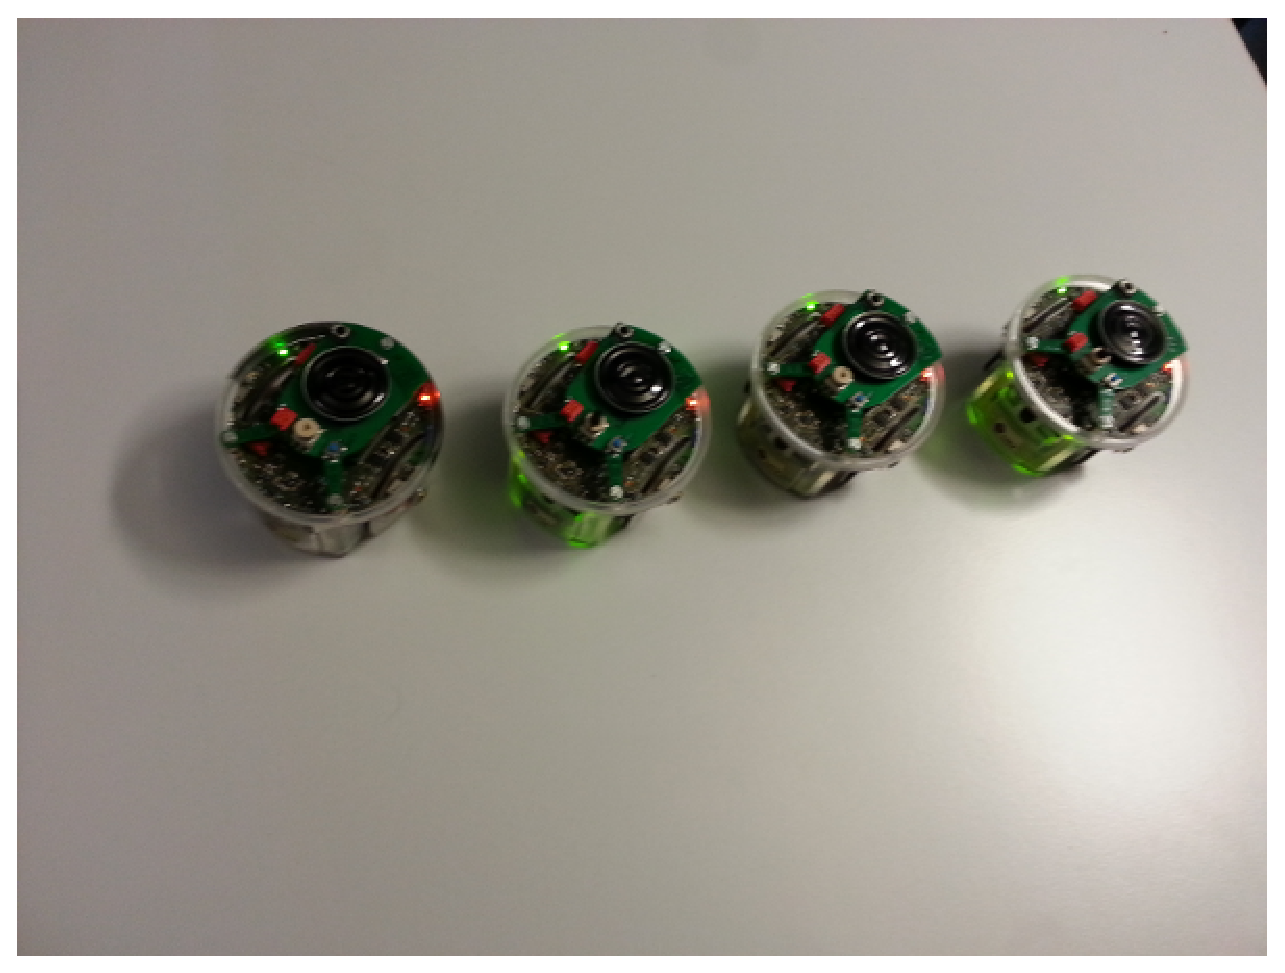
\includegraphics[scale=0.5]{pics/epucks_2.eps} 
\caption{The orange light is visible on each e-puck}
\end{figure}

After we checked the bluetooth connection, we pushed the reset button on each e-puck.

\subsubsection*{Step 9}
In this step we were stuck. As mentioned in the section "Our troubles" aseba studio didn't show a tab for each connectd e-puck.

\newpage
\subsection*{Conclusion}
We spent almost two hours to solve the problems in step 9, but we didn't succeed in troubleshooting ;-).

As we know since last friday, we weren't the only ones with the same problem.


\end{document}
